\subsection{Additive Dice-Bce-NQM Loss}
\label{experiments:02.1:diceBce+NQM}
\begin{figure}[h!]
    \vspace{0.5cm}
    \centering
        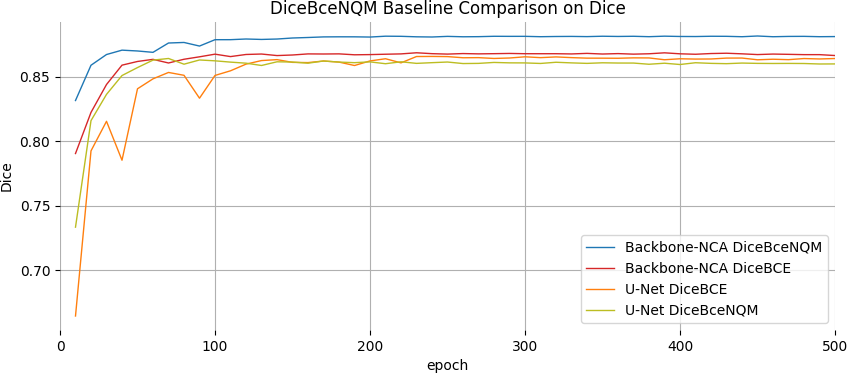
\includegraphics[width=\linewidth]{Graphics/Experiments/2.1_inverted_freeAxes_Loss_DiceLoss()_test_mask0.png}
        \caption{Backbone-NCA trained on DiceBceNQM (blue). For comparison, as baselines, a Backbone-NCA trained on DiceBCE and two U-Nets are given. The convergence of the Backbone-NCA on DiceBceNQM is quite similar to the Baselines. Therefore, training is stable on this loss regarding the Dice score. The U-Nets have been trained for 1000 epochs in total, but the Dice does not change any further, even so the train loss does.}
    \label{fig:02.1:DiceBceNQM:Baselines:onDice}
\end{figure}

As we have seen in \autoref{experiments:01.0:Into}, using only the NQM as a loss function cannot work because the reference to the ground truth label is missing, and since the models we use, the Backbone-NCA as well as the Med-NCA, already use a well working loss; the DiceBCE given in \ref{DiceBCE-Loss} is close to it, to go from there. In this way, we have developed a working NQM-loss function, which works as well as the DiceBce in our first tests, just by adding the NQM to the DiceBCE. The DiceBceNQM, as we later used it mainly for our robustness improvement experiments.

Since the NQM can be very large in the initial training cycles, we additionally cropped the NQM to a value of $\in(0,1)$ to relax the weight of the NQM in the total loss. This results in the DiceBceNQM as follows:

\begin{align}
    \text{DiceBceNQM} &:= 1 - \mathrm{Dice} + \mathrm{Bce} {\color{red}+} \mathrm{NQM},\label{eq:02.1:DiceBceNQM}\\           
    \mathrm{NQM}\ &:=\ \min\left(1, \quad \frac{\sum_{s\in SD} (s) +1} {\sum_{m\in\mu} +1}\right), \qquad
    SD = \sqrt{\frac{\sum^N_{i=1}(v_i-\mu)^2}  {N}  \varepsilon}, \qquad
    \mu = \frac{\sum^N_{i=1}v_i}  {N}               \label{eq:02.1:Only_NQM}
\end{align}

As can be seen in \autoref{fig:02.1:DiceBceNQM:Baselines:onDice} (for Dice), \autoref{fig:02.1:DiceBceNQM:Baselines:onTrainLoss} (for train losses), the Backbone-NCA converges on the DiceBceNQM about as well as on the DiceBCE, measured on Dice, or even slightly better (+1.8 points). We also trained two U-Nets, one on the DiceBCE, the other on the DiceBceNQM, as additional baselines. The convergence is approximately similar to the Backbone-NCA trained on DiceBCE. Furthermore \autoref{fig:02.1:DiceBceNQM:Baselines:Segmentations} show segmentations for the final model and baselines. As can be seen by eye the predictions with the DiceBceNQM are as good as with the DiceBCE. Putting all this together, training on this loss is stable and reliable and as least as good as on the DiceBCE alone. Therefor we used it for most of our robustness tests in \autoref{experiments:03.0:Intro}. 

\begin{figure}[h!]
    \vspace{0.5cm}
    \centering
        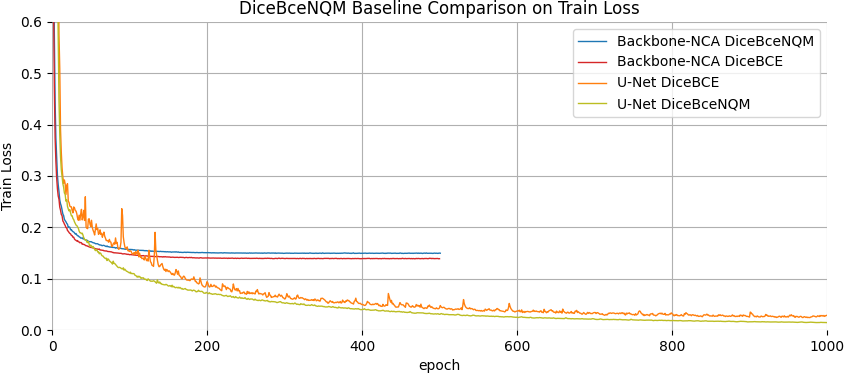
\includegraphics[width=\linewidth]{Graphics/Experiments/2.1_train_loss_freeAxes_Loss_train_0.png}
        \caption{Backbone-NCA trained on DiceBceNQM (blue). For comparison, as baselines, a Backbone-NCA trained on DiceBCE and two U-Nets are given. The convergence of the Backbone-NCA on DiceBceNQM is quite similar to the Baselines. Therefore, training is stable on this loss regarding. The U-Nets have been trained for 1000 epochs in total, Backbone-NCAs only 500 epochs.}
    \label{fig:02.1:DiceBceNQM:Baselines:onTrainLoss}
\end{figure}

\begin{figure}[h!]
    \vspace{0.5cm}
    \centering
        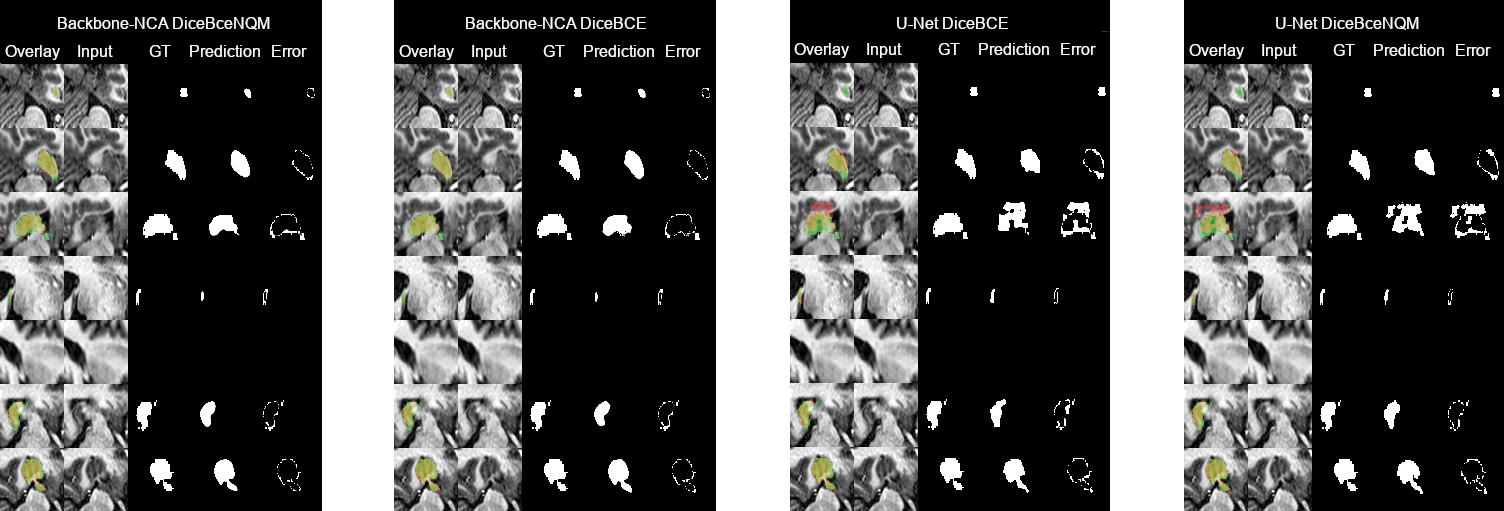
\includegraphics[width=\linewidth]{Graphics/Experiments/2.1_BaselineComparison.png}
        \caption{Backbone-NCA trained on DiceBceNQM (left). For comparison, as baselines, a Backbone-NCA trained on DiceBCE and two U-Nets are given. For each model the same image volumes (inputs) are given. With ground truth labels (GT), predictions, and errors. The overlay shows the input image with false positive (red), true positive (yellow), and  false negative (green). All for the final models after 500 epochs for Backbone-NCAs and 1000 epochs for U-Nets. First and foremost the predictions with the DiceBceNQM for the Backbone-NCA are at least as good as with the DiceBCE. Therefor training on the DiceBceNQM is stable. Even so some segmentations by the U-Nets look worse, then by the Backbone-NCAs, the Dice is is quite similar (\autoref{fig:02.1:DiceBceNQM:Baselines:onDice}).}
    \label{fig:02.1:DiceBceNQM:Baselines:Segmentations}
\end{figure}


We also tested different stacksizes and alpha-values, like in \autoref{experiments:03.1.0:backbone_hippo:intro} and here even in more configurations then there, but since, they did not show any effect here (but there), they are introduced in \autoref{experiments:03.1.0:backbone_hippo:intro}.